% ============================================================
% Semester Project Template
% Object Oriented Programming using C++
% Institute of Business Administration Karachi
% ============================================================

\documentclass[11pt]{article}

% ── Packages ──────────────────────────────────────────────────────────────
\usepackage[a4paper, margin=1in]{geometry}
\usepackage[utf8]{inputenc}
\usepackage[T1]{fontenc}
\usepackage{amsmath, amssymb, amsthm}
\usepackage{graphicx}
\usepackage{hyperref}
\usepackage{listings}
\usepackage{xcolor}
\usepackage{titlesec}
\usepackage{fancyhdr}
\usepackage{parskip}
\usepackage{caption}
\usepackage{subcaption}
\usepackage{booktabs}
\usepackage{array}
\usepackage{enumitem}
\usepackage{float}
\usepackage{tikz}
\usepackage{tcolorbox}
\tcbuselibrary{skins,breakable}
\usetikzlibrary{shapes,arrows,positioning,fit,backgrounds,calc}

% ── Colours ───────────────────────────────────────────────────────────────
\definecolor{primary}{RGB}{165, 28, 48}       % IBA crimson
\definecolor{secondary}{RGB}{0, 53, 107}      % navy
\definecolor{accent}{RGB}{232, 95, 26}        % orange
\definecolor{codebg}{RGB}{245, 248, 250}
\definecolor{codecomment}{RGB}{106, 153, 85}
\definecolor{codekeyword}{RGB}{0, 0, 200}
\definecolor{codestring}{RGB}{163, 21, 21}
\definecolor{stdtype}{RGB}{43, 145, 175}

% ── C++ Listing style ─────────────────────────────────────────────────────
\lstdefinestyle{cpp}{
    language=C++,
    backgroundcolor=\color{codebg},
    basicstyle=\ttfamily\small,
    breaklines=true,
    captionpos=b,
    commentstyle=\color{codecomment}\itshape,
    keywordstyle=\color{codekeyword}\bfseries,
    stringstyle=\color{codestring},
    numbers=left,
    numbersep=8pt,
    numberstyle=\tiny\color{gray},
    frame=single,
    rulecolor=\color{gray!40},
    showstringspaces=false,
    tabsize=4,
    xleftmargin=1.5em,
    framexleftmargin=1.5em,
    morekeywords={override, nullptr, auto, decltype, noexcept,
                  final, constexpr, explicit, virtual, class, struct,
                  public, private, protected, new, delete, this},
}
\lstset{style=cpp}

% ── Header / Footer ───────────────────────────────────────────────────────
\pagestyle{fancy}
\fancyhf{}
\renewcommand{\headrulewidth}{0.4pt}
\fancyhead[L]{\textcolor{primary}{\textbf{\mytitle}}}
\fancyhead[R]{\textcolor{primary}{\thepage}}

\fancypagestyle{firstpage}{
    \fancyhf{}
    \renewcommand{\headrulewidth}{0pt}
    \fancyfoot[C]{\textcolor{gray}{\small \mytitle\ -- \thepage}}
}

% ── Section formatting ────────────────────────────────────────────────────
\titleformat{\section}
    {\normalfont\Large\bfseries\color{primary}}{\thesection}{1em}{}
\titleformat{\subsection}
    {\normalfont\large\bfseries\color{secondary}}{\thesubsection}{1em}{}
\titleformat{\subsubsection}
    {\normalfont\normalsize\bfseries\color{accent}}{\thesubsubsection}{1em}{}

% ── TikZ node styles ──────────────────────────────────────────────────────
\tikzset{
    block/.style={rectangle, draw, fill=blue!10, text width=2.5cm,
                  text centered, rounded corners, minimum height=1cm},
    io/.style={trapezium, trapezium left angle=70, trapezium right angle=110,
               draw, fill=red!10, text width=2cm, text centered, minimum height=1cm},
    process/.style={rectangle, draw, fill=green!10, text width=2.5cm,
                    text centered, rounded corners, minimum height=1cm},
    decision/.style={diamond, draw, fill=yellow!10, text width=2cm,
                     text centered, aspect=2, minimum height=1cm},
    line/.style={draw, -latex},
}

% ── Info boxes ────────────────────────────────────────────────────────────
\newtcolorbox{infobox}{
    colback=primary!5, colframe=primary, boxrule=0.6pt,
    arc=3pt, left=8pt, right=8pt, top=6pt, bottom=6pt, breakable
}
\newtcolorbox{notebox}{
    colback=accent!5, colframe=accent, boxrule=0.6pt,
    arc=3pt, left=8pt, right=8pt, top=6pt, bottom=6pt, breakable
}

% ── Project metadata (edit these) ─────────────────────────────────────────
\newcommand{\mytitle}{Semester Project: [Your Project Title]}
\newcommand{\mycourse}{CSE142 Object Oriented Programming Techniques}
\newcommand{\mysemester}{Spring 2026}
\newcommand{\myinstructor}{[Instructor Name]}
\newcommand{\authorone}{[Student Name 1] --- ERP: [XXXXX]}
\newcommand{\authortwo}{[Student Name 2] --- ERP: [XXXXX]}   % leave blank if solo
\newcommand{\authorthree}{}                                    % leave blank if not needed
\newcommand{\duedate}{[Date]}

% ─────────────────────────────────────────────────────────────────────────
\begin{document}
% ─────────────────────────────────────────────────────────────────────────

% ── Title page ────────────────────────────────────────────────────────────
\thispagestyle{firstpage}
\begin{center}
    \vspace*{0.5cm}

    {\Huge\bfseries\textcolor{primary}{\mytitle}}

    \vspace{0.5cm}
    \rule{0.9\textwidth}{1pt}
    \vspace{0.5cm}

    {\Large A Semester Project Report}

    \vspace{1cm}

    \begin{tabular}{rl}
        \textbf{Course:}     & \mycourse     \\[4pt]
        \textbf{Semester:}   & \mysemester   \\[4pt]
        \textbf{Instructor:} & \myinstructor \\[4pt]
        \textbf{Due Date:}   & \duedate      \\[4pt]
        \textbf{Author(s):}  & \authorone    \\[2pt]
                             & \authortwo    \\[2pt]
                             & \authorthree  \\
    \end{tabular}

    \vspace{1.5cm}

    
\includegraphics[width=0.5\textwidth]{misc/IBA-logo}

    \vfill

    {\large Department of Computer Science}\\[4pt]
    {\large Institute of Business Administration, Karachi}\\[6pt]
    \today
\end{center}

\newpage

% ── Abstract ──────────────────────────────────────────────────────────────
\section*{Abstract}
\addcontentsline{toc}{section}{Abstract}

Write a concise summary of your project here (150--250 words). Cover:
\begin{itemize}
    \item The problem being solved
    \item Your approach and OOP design choices
    \item Key C++ features used (inheritance, polymorphism, templates, etc.)
    \item Results and conclusions
\end{itemize}

\vspace{0.3cm}
\noindent\textbf{Keywords:} [e.g., Object-Oriented Programming, C++, Inheritance, Polymorphism, \ldots]

\newpage

% ── Table of contents ─────────────────────────────────────────────────────
\tableofcontents
\newpage

% ─────────────────────────────────────────────────────────────────────────
\section{Introduction}
% ─────────────────────────────────────────────────────────────────────────

\subsection{Background}
Provide background information on the problem domain. Explain why this project is important and how it relates to Object-Oriented Programming principles taught in \mycourse.

\subsection{Problem Statement}
Clearly state the problem you are addressing:
\begin{itemize}
    \item What is the specific problem?
    \item Why is it challenging?
    \item What are the inputs, outputs, and constraints?
\end{itemize}

\subsection{Objectives}
List the main objectives of this project:
\begin{enumerate}
    \item Design a class hierarchy that models the problem domain.
    \item Implement core OOP concepts: encapsulation, inheritance, and polymorphism.
    \item Demonstrate correct use of constructors, destructors, and operator overloading.
    \item[4.] \textit{[Add your own specific objective.]}
\end{enumerate}

\subsection{Scope and Limitations}
Define what is included in this project and what falls outside its scope.

\begin{notebox}
Be explicit about assumptions and constraints. For example: ``All input is assumed to be valid'', or ``Only ASCII characters are supported''.
\end{notebox}

% ─────────────────────────────────────────────────────────────────────────
\section{OOP Design}
% ─────────────────────────────────────────────────────────────────────────

\subsection{Class Hierarchy}
Describe and diagram the class hierarchy you designed. Explain which relationships are \emph{inheritance} (is-a) and which are \emph{composition} (has-a).

\begin{figure}[H]
    \centering
    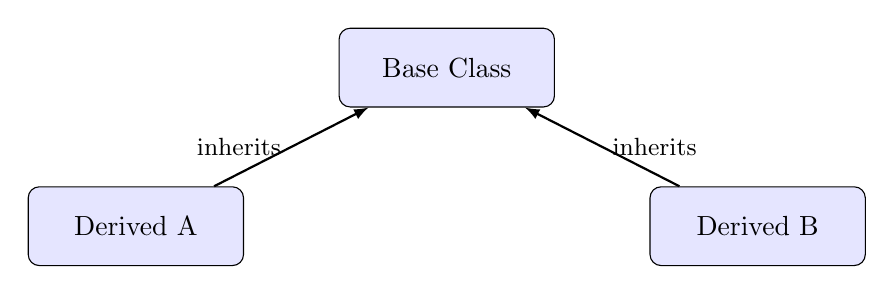
\begin{tikzpicture}[node distance=1.8cm]
        \node [block] (base)   {Base Class};
        \node [block, below left=1cm and 1.2cm of base]  (derived1) {Derived A};
        \node [block, below right=1cm and 1.2cm of base] (derived2) {Derived B};
        \draw[-latex, thick] (derived1) -- (base) node[midway, left, font=\small]{inherits};
        \draw[-latex, thick] (derived2) -- (base) node[midway, right, font=\small]{inherits};
    \end{tikzpicture}
    \caption{Class hierarchy diagram}
    \label{fig:hierarchy}
\end{figure}

\subsection{Class Descriptions}
For each class, describe its responsibilities, member variables, and key methods.

\begin{table}[H]
    \centering
    \caption{Summary of Classes}
    \label{tab:classes}
    \begin{tabular}{|l|p{4cm}|p{5cm}|}
        \hline
        \textbf{Class} & \textbf{Responsibility} & \textbf{Key Members} \\
        \hline
        \texttt{BaseClass}    & [Describe role] & \texttt{member1, method1()} \\
        \hline
        \texttt{DerivedClassA} & [Describe role] & \texttt{member2, method2()} \\
        \hline
        \texttt{DerivedClassB} & [Describe role] & \texttt{member3, method3()} \\
        \hline
    \end{tabular}
\end{table}

\subsection{OOP Concepts Applied}
Explain which OOP features your design uses and \emph{why}:

\begin{itemize}
    \item \textbf{Encapsulation:} Private/protected members accessed through public getters/setters.
    \item \textbf{Inheritance:} [Which classes inherit from which and why.]
    \item \textbf{Polymorphism:} Virtual functions allow \ldots
    \item \textbf{Operator Overloading:} \texttt{operator<<}, \texttt{operator+}, etc.
    \item \textbf{Templates (if used):} [Explain any generic classes or functions.]
\end{itemize}

% ─────────────────────────────────────────────────────────────────────────
\section{Implementation}
% ─────────────────────────────────────────────────────────────────────────

\subsection{Development Environment}
\begin{itemize}
    \item \textbf{Language:} C++17
    \item \textbf{Compiler:} g++ / MSVC / Clang (state which)
    \item \textbf{IDE:} [VS Code / CLion / Visual Studio / other]
    \item \textbf{Build system:} [Makefile / CMake / manual]
    \item \textbf{Platform:} [Windows / Linux / macOS]
\end{itemize}

\subsection{Base Class}

\begin{lstlisting}[caption={Base class definition and implementation}]
#include <iostream>
#include <string>
using namespace std;

class Animal {
private:
    string name;
    int    age;

public:
    // Constructor
    Animal(const string& n, int a) : name(n), age(a) {}

    // Virtual destructor (essential for polymorphism)
    virtual ~Animal() { cout << "Animal destroyed\n"; }

    // Pure virtual function -> makes Animal abstract
    virtual void speak() const = 0;

    // Virtual function with default behaviour
    virtual void display() const {
        cout << "Name: " << name << ", Age: " << age << "\n";
    }

    // Getters
    string getName() const { return name; }
    int    getAge()  const { return age;  }

    // Operator overloading
    friend ostream& operator<<(ostream& os, const Animal& a) {
        os << "Animal[" << a.name << ", " << a.age << "]";
        return os;
    }
};
\end{lstlisting}

\subsection{Derived Classes}

\begin{lstlisting}[caption={Derived class with overridden virtual functions}]
class Dog : public Animal {
private:
    string breed;

public:
    Dog(const string& name, int age, const string& breed)
        : Animal(name, age), breed(breed) {}

    ~Dog() override { cout << "Dog destroyed\n"; }

    // Override the pure virtual function
    void speak() const override {
        cout << getName() << " says: Woof!\n";
    }

    // Override display to add breed information
    void display() const override {
        Animal::display();           // call base version first
        cout << "Breed: " << breed << "\n";
    }

    string getBreed() const { return breed; }
};

class Cat : public Animal {
public:
    Cat(const string& name, int age) : Animal(name, age) {}

    void speak() const override {
        cout << getName() << " says: Meow!\n";
    }
};
\end{lstlisting}

\subsection{Demonstrating Polymorphism}

\begin{lstlisting}[caption={Using base class pointers for polymorphic behaviour}]
int main() {
    // Array of base class pointers (polymorphism)
    Animal* animals[3];
    animals[0] = new Dog("Rex",    4, "German Shepherd");
    animals[1] = new Cat("Whiskers", 2);
    animals[2] = new Dog("Buddy",  6, "Labrador");

    // Virtual dispatch: correct speak() called at runtime
    for (int i = 0; i < 3; i++) {
        animals[i]->display();
        animals[i]->speak();
        cout << "---\n";
    }

    // Clean up (virtual destructor ensures correct deletion)
    for (int i = 0; i < 3; i++)
        delete animals[i];

    return 0;
}
\end{lstlisting}

\textbf{Expected output:}
\begin{tcolorbox}[colback=black!88, coltext=green!80,
                  fontupper=\ttfamily\small, boxrule=0pt, arc=2pt]
Name: Rex, Age: 4\\
Breed: German Shepherd\\
Rex says: Woof!\\
---\\
Name: Whiskers, Age: 2\\
Whiskers says: Meow!\\
---\\
Name: Buddy, Age: 6\\
Breed: Labrador\\
Buddy says: Woof!\\
---
\end{tcolorbox}

\subsection{Additional Key Functions}
Add more code snippets here for other important parts of your implementation. Include any:
\begin{itemize}
    \item Copy constructor / copy assignment operator
    \item Move constructor / move assignment operator (Rule of Five)
    \item Operator overloads (\texttt{+}, \texttt{==}, \texttt{<}, etc.)
    \item Template classes or functions
    \item File I/O routines
\end{itemize}

\begin{lstlisting}[caption={Example: overloaded comparison operator}]
bool operator<(const Animal& other) const {
    return this->getAge() < other.getAge();
}
\end{lstlisting}

% ─────────────────────────────────────────────────────────────────────────
\section{Testing}
% ─────────────────────────────────────────────────────────────────────────

\subsection{Test Cases}

\begin{table}[H]
    \centering
    \caption{Test Cases and Results}
    \label{tab:tests}
    \renewcommand{\arraystretch}{1.3}
    \begin{tabular}{|c|p{3.5cm}|p{3.5cm}|p{2.5cm}|c|}
        \hline
        \textbf{TC \#} & \textbf{Input / Action} & \textbf{Expected Output} & \textbf{Actual Output} & \textbf{Pass?} \\
        \hline
        TC-01 & Create \texttt{Dog("Rex", 4, "Husky")} & Object created correctly & As expected & \checkmark \\
        \hline
        TC-02 & Call \texttt{speak()} via \texttt{Animal*} & \texttt{"Rex says: Woof!"} & As expected & \checkmark \\
        \hline
        TC-03 & Delete via base pointer & Both destructors called & As expected & \checkmark \\
        \hline
        TC-04 & \textit{[Your test case]} & \textit{[Expected]} & \textit{[Actual]} & \\
        \hline
        TC-05 & \textit{[Your test case]} & \textit{[Expected]} & \textit{[Actual]} & \\
        \hline
    \end{tabular}
\end{table}

\subsection{Edge Cases}
Describe edge cases you tested:
\begin{itemize}
    \item Empty input / null pointers
    \item Boundary values
    \item Copying / moving objects
    \item Exceptions thrown and caught
\end{itemize}

% ─────────────────────────────────────────────────────────────────────────
\section{Results and Discussion}
% ─────────────────────────────────────────────────────────────────────────

\subsection{Results}
Summarise what your program produces. Include screenshots, console output, or performance tables.

\begin{table}[H]
    \centering
    \caption{Performance / Benchmark Results}
    \label{tab:perf}
    \begin{tabular}{lccc}
        \toprule
        \textbf{Operation} & \textbf{Input Size} & \textbf{Time (ms)} & \textbf{Notes} \\
        \midrule
        Insert   & 100    & 0.12 & \\
        Insert   & 10,000 & 8.45 & \\
        Search   & 10,000 & 1.23 & Binary search \\
        Delete   & 10,000 & 2.34 & \\
        \bottomrule
    \end{tabular}
\end{table}

\subsection{Analysis}
\begin{itemize}
    \item Did your implementation meet the design objectives?
    \item Compare actual complexity against theoretical $O(\cdot)$ bounds.
    \item Discuss any unexpected behaviour or limitations.
\end{itemize}

% ─────────────────────────────────────────────────────────────────────────
\section{Challenges and Solutions}
% ─────────────────────────────────────────────────────────────────────────

\subsection{Challenge 1: [Name]}
\textbf{Problem:} [Describe the issue encountered.]\\
\textbf{Solution:} [Explain how you resolved it.]\\
\textbf{Learning:} [What did you take away from it?]

\subsection{Challenge 2: [Name]}
\textbf{Problem:} [Describe the issue encountered.]\\
\textbf{Solution:} [Explain how you resolved it.]\\
\textbf{Learning:} [What did you take away from it?]

% ─────────────────────────────────────────────────────────────────────────
\section{Future Work}
% ─────────────────────────────────────────────────────────────────────────

Possible extensions and improvements:
\begin{itemize}
    \item Add a GUI / menu-driven interface.
    \item Persist data to files using serialisation.
    \item Introduce templates to generalise containers.
    \item Add unit testing with a framework such as Google Test.
\end{itemize}

% ─────────────────────────────────────────────────────────────────────────
\section{Conclusion}
% ─────────────────────────────────────────────────────────────────────────

Summarise the project's contributions and reflect on what you learned.

\begin{infobox}
A strong conclusion should:
\begin{itemize}
    \item Restate the problem and your OOP design approach.
    \item Summarise key results and test outcomes.
    \item Reflect on which OOP concepts were most useful.
    \item Suggest next steps or broader implications.
\end{itemize}
\end{infobox}

% ─────────────────────────────────────────────────────────────────────────
\newpage
\section*{References}
\addcontentsline{toc}{section}{References}
% ─────────────────────────────────────────────────────────────────────────

List references in IEEE format. Example entries:

\begin{enumerate}[label={[\arabic*]}]
    \item B. Stroustrup, \textit{The C++ Programming Language}, 4th ed. Addison-Wesley, 2013.
    \item S. Meyers, \textit{Effective Modern C++}. O'Reilly Media, 2014.
    \item \textit{cppreference.com}. [Online]. Available: \url{https://en.cppreference.com}. [Accessed: \today].
    \item \textit{[Add your own references here.]}
\end{enumerate}

% ─────────────────────────────────────────────────────────────────────────
\newpage
\appendix
\section{Complete Source Code}
\label{sec:code}
% ─────────────────────────────────────────────────────────────────────────

Paste your complete C++ source files below. Replace the examples with your actual code.

\subsection{main.cpp}
\begin{lstlisting}[caption={main.cpp --- entry point}]
#include <iostream>
#include "Animal.h"
#include "Dog.h"
#include "Cat.h"
using namespace std;

int main() {
    // Your full main() code goes here
    cout << "Hello from your OOP project!\n";
    return 0;
}
\end{lstlisting}

\subsection{Animal.h}
\begin{lstlisting}[caption={Animal.h --- base class header}]
#pragma once
#include <string>
#include <iostream>
using namespace std;

class Animal {
    // Paste your full class header here
};
\end{lstlisting}

\subsection{Dog.h / Dog.cpp}
\begin{lstlisting}[caption={Dog.h --- derived class header}]
#pragma once
#include "Animal.h"

class Dog : public Animal {
    // Paste your full class header here
};
\end{lstlisting}

\section{Installation and Usage}
\label{sec:install}

\subsection{Prerequisites}
\begin{itemize}
    \item C++17-compatible compiler: \texttt{g++ 9+} or MSVC 2019+
    \item \textit{Optional:} CMake 3.15+ for build automation
\end{itemize}

\subsection{Compilation}
\begin{lstlisting}[language=bash, caption={Building with g++}]
# Compile all source files
g++ -std=c++17 -Wall -o project main.cpp Animal.cpp Dog.cpp Cat.cpp

# Run the program
./project
\end{lstlisting}

\subsection{Usage Examples}
\begin{lstlisting}[language=bash, caption={Running the program}]
# Basic run
./project

# With optional arguments (if your program supports them)
./project --input data.txt
\end{lstlisting}

\end{document}